\chapter{Grafische Nutzeroberfläche}
\label{a:gui}

%\section{Verwendete Abk"urzungen}

\begin{figure}[H]
\centering
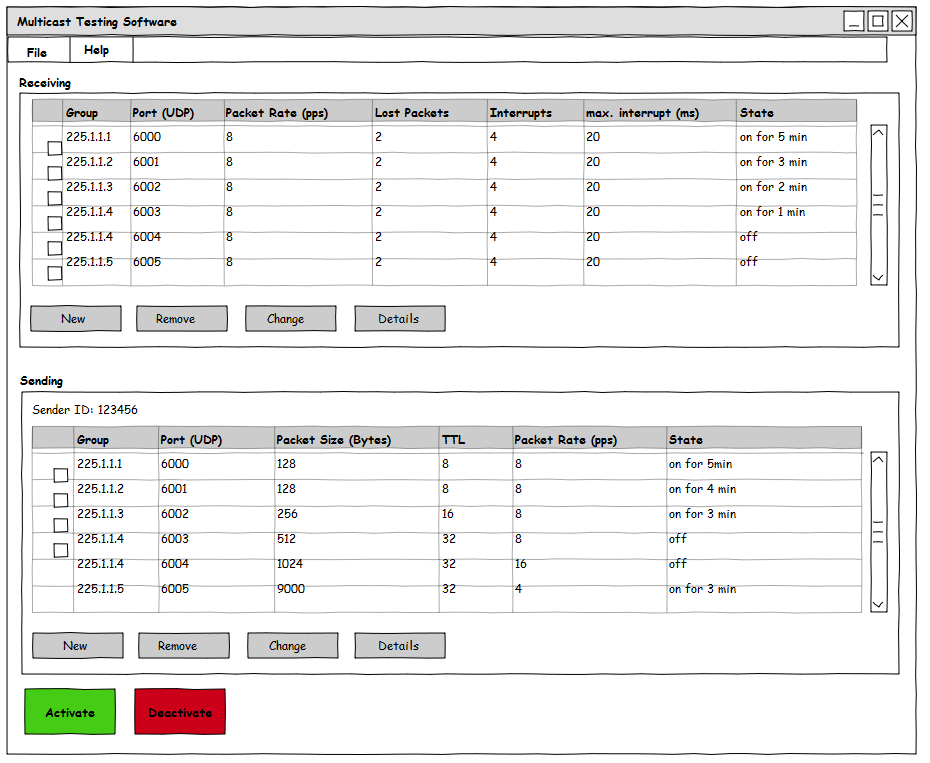
\includegraphics[scale=0.5]{images/gui/main.png}
\caption{Hauptprogramm}
\end{figure}
Die Standart-Ansicht des Programms zeigt eine Auflistung aller aus- und
eingehenden Datenströme. Nach Anforderungen werden alle relevanten
Informationen auf einen Blick angezeigt und es können bequem mehrere Ströme auf
einmal bearbeitet werden.

\begin{figure}[H]
\centering
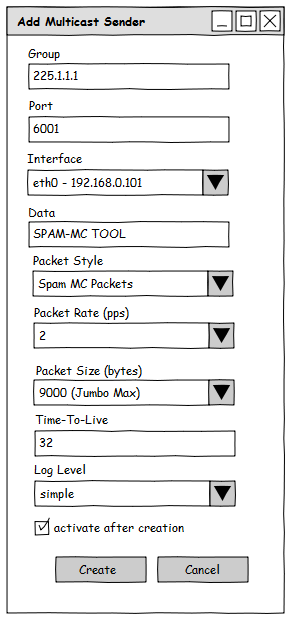
\includegraphics[scale=0.5]{images/gui/addsender.png}
\caption{Hinzufügen eines Senders}
\end{figure}
Beim Hinzufügen eines neuen Senders werden alle benötigten Werte vom Benutzer
erfragt. Bei seiner Auswahlt wird er durch Vorschläge und Eingrenzungen des
Programms unterstützt.

\begin{figure}[H]
\centering
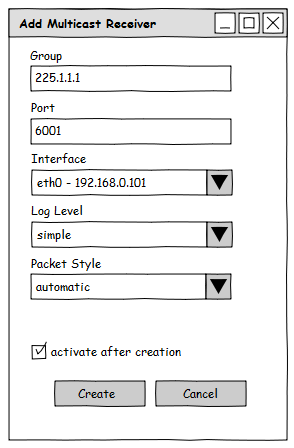
\includegraphics[scale=0.5]{images/gui/addrec.png}
\caption{Hinzufügen eines Empfängers}
\end{figure}
Das Hinzufügen eines neuen Empfängers analog zu oben.

\begin{figure}[H]
\centering
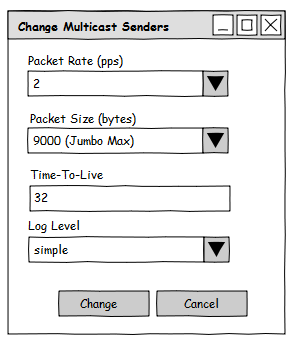
\includegraphics[scale=0.5]{images/gui/changesender.png}
\caption{Ändern eines Senders}
\end{figure}
Beim Umkonfigurieren von Sendern können bei Mehrfachauswahl sinnvolle Parameter
bequem für alle Datenströme auf einmal geändert werden.

\begin{figure}[H]
\centering
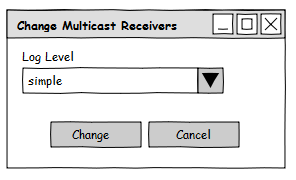
\includegraphics[scale=0.5]{images/gui/changerec.png}
\caption{Ändern eines Empfängers}
\end{figure}
Das Umkonfigurieren von Empfängern analog zu oben.

\begin{figure}[H]
\centering
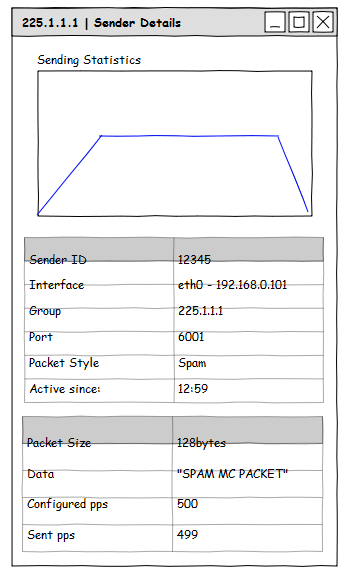
\includegraphics[scale=0.5]{images/gui/detailssender.png}
\caption{Detailansicht eines Senders}
\end{figure}
Benötigt man genauere Informationen zu einem bestimmten Datenstrom, kann man
sich eine detaillierte Sicht anzeigen lassen. In dieser werden alle vorhandenen
Informationen dargestellt. Zu Beachten: Die graphische Darstellung der
Datenströme ist eine optionale Anforderung, ihre Implementierung in Version 1
ist noch nicht sicher.

\begin{figure}[H]
\centering
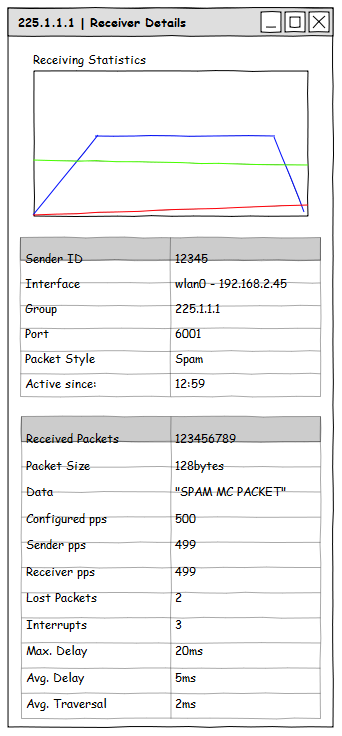
\includegraphics[scale=0.5]{images/gui/detailsrec.png}
\caption{Detailansicht eines Empfängers}
\end{figure}
Detailansicht eines Empfängers analog zu oben.

\begin{figure}[H]
\centering

\includegraphics[scale=0.5]{images/gui/error.png}
\caption{Beispiel für Fehleranzeige}
\end{figure}
Bei falschen Eingaben oder Programmfehlern wird em Nutzer eine einfach
verständliche und eindeutige Fehlermeldung angezeigt.
